\documentclass{article}
\usepackage{graphicx}
\usepackage{amsmath}
\usepackage[parfill]{parskip}
\usepackage{hyperref}
\usepackage{tikz}
\graphicspath{ {./figures/} }

\usepackage{biblatex}
\addbibresource{references.bib}

\title{COMP.SEC.220 Security Protocol\footnote{github --- \url{https://github.com/ancuongnguyen07/SecurityProtocol}}}
\author{Cuong Nguyen --- Coursework 1}
\date{22/04/2022}

\begin{document}
    
\maketitle

\section*{Exercise 1 --- XOR Encryption}
%
Given a message \emph{m} and the OTP encryption \emph{c}, we \textbf{can} compute
the OTP key \emph{k} by XORing the plaintext \emph{m} and the ciphertext \emph{c}.
The ciphertext is given by:

\begin{align*}
    c = m \oplus k,
\end{align*}

therefore, we can easily compute the \emph{k} by:

\begin{align*}
    k = c \oplus m,
\end{align*}

where \emph{c} and \emph{m} are known.

\section*{Exercise 2 --- Substitution Cipher}
%

\section*{Exercise 3 --- Diffie-Hellman}
%
\subsection*{a)}
Alice's intermediate values:

\begin{align*}
    X &= g^{a} \mod p\\
    X &= 7^6 \mod 11\\
    X &= 4 \mod 11
\end{align*}

Bob's intermediate values:

\begin{align*}
    Y &= g^{b} \mod p\\
    Y &= 7^9 \mod 11\\
    Y &= 8 \mod 11
\end{align*}

The final key that Alice and Bob exchange:

\begin{align*}
    K_{AB} &= X^b \mod p\\
    K_{AB} &= 4^9 \mod 11\\
    K_{AB} &= 3 \mod 11
\end{align*}

\subsection*{b)}
Since \(g=7\) is the primitive root of \(p=11\) so we can brute-force
\emph{a} in \(g^a = 5 \mod 11\) in at most 10 trials. Hence, the secret
value of Alice \emph{a} is 2. The secret value of Bob \emph{b}, which is 5, can be
computed by the same approach. Thus, the final key that Alice and Bob exchanged
is given by:

\begin{align*}
    K_{AB} &= X^b = Y^a = g^{ab} \mod p\\
    K_{AB} &= 1 \mod 11 
\end{align*}

\subsection*{c)}
By running the Caesar decryption script with the shift key is 1 (left-shift 1
in this case. In other words, it is right-shift 25), I obtained the plaintext:

\begin{center}
    \textbf{SUEDE JACKET WITH CANDY STRIPE LINING}
\end{center}


\section*{Exercise 4 --- Three party Diffie-Hellman}
%
Waiting for the TA's feedback

\section*{Exercise 5 --- Symmetric Encryption}
%
\begin{figure}
    \centering

    \tikzset{every picture/.style={line width=0.75pt}} %set default line width to 0.75pt        

    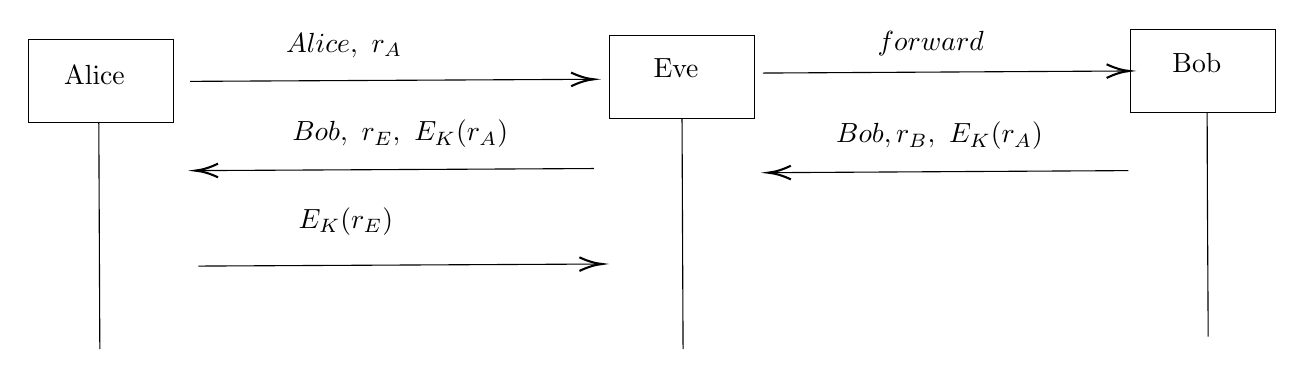
\begin{tikzpicture}[x=0.75pt,y=0.75pt,yscale=-1,xscale=1]
    %uncomment if require: \path (0,230); %set diagram left start at 0, and has height of 230

    %Shape: Rectangle [id:dp1743019806713867] 
    \draw   (32,32) -- (102,32) -- (102,72) -- (32,72) -- cycle ;

    %Shape: Rectangle [id:dp6293669652442805] 
    \draw   (563,27) -- (633,27) -- (633,67) -- (563,67) -- cycle ;

    %Shape: Rectangle [id:dp9205463275779588] 
    \draw   (312,30) -- (382,30) -- (382,70) -- (312,70) -- cycle ;

    %Straight Lines [id:da9822614621505796] 
    \draw    (110,52) -- (302.5,51.01) ;
    \draw [shift={(304.5,51)}, rotate = 179.71] [color={rgb, 255:red, 0; green, 0; blue, 0 }  ][line width=0.75]    (10.93,-3.29) .. controls (6.95,-1.4) and (3.31,-0.3) .. (0,0) .. controls (3.31,0.3) and (6.95,1.4) .. (10.93,3.29)   ;
    %Straight Lines [id:da8180326777766349] 
    \draw    (66,72) -- (66.5,181) ;
    %Straight Lines [id:da7527020702065276] 
    \draw    (347,70) -- (347.5,181) ;
    %Straight Lines [id:da7872518105548856] 
    \draw    (600,67) -- (600.1,102) -- (600.5,175) ;
    %Straight Lines [id:da6977144240055365] 
    \draw    (386,48) -- (560.5,47.01) ;
    \draw [shift={(562.5,47)}, rotate = 179.68] [color={rgb, 255:red, 0; green, 0; blue, 0 }  ][line width=0.75]    (10.93,-3.29) .. controls (6.95,-1.4) and (3.31,-0.3) .. (0,0) .. controls (3.31,0.3) and (6.95,1.4) .. (10.93,3.29)   ;
    %Straight Lines [id:da6481231910605018] 
    \draw    (562,95) -- (390.5,95.99) ;
    \draw [shift={(388.5,96)}, rotate = 359.67] [color={rgb, 255:red, 0; green, 0; blue, 0 }  ][line width=0.75]    (10.93,-3.29) .. controls (6.95,-1.4) and (3.31,-0.3) .. (0,0) .. controls (3.31,0.3) and (6.95,1.4) .. (10.93,3.29)   ;
    %Straight Lines [id:da28842039284308707] 
    \draw    (304.5,94) -- (114.5,94.99) ;
    \draw [shift={(112.5,95)}, rotate = 359.7] [color={rgb, 255:red, 0; green, 0; blue, 0 }  ][line width=0.75]    (10.93,-3.29) .. controls (6.95,-1.4) and (3.31,-0.3) .. (0,0) .. controls (3.31,0.3) and (6.95,1.4) .. (10.93,3.29)   ;
    %Straight Lines [id:da5471284771409243] 
    \draw    (114,141) -- (306.5,140.01) ;
    \draw [shift={(308.5,140)}, rotate = 179.71] [color={rgb, 255:red, 0; green, 0; blue, 0 }  ][line width=0.75]    (10.93,-3.29) .. controls (6.95,-1.4) and (3.31,-0.3) .. (0,0) .. controls (3.31,0.3) and (6.95,1.4) .. (10.93,3.29)   ;

    % Text Node
    \draw (48,43) node [anchor=north west][inner sep=0.75pt]   [align=left] {Alice};
    % Text Node
    \draw (582,37) node [anchor=north west][inner sep=0.75pt]   [align=left] {Bob};
    % Text Node
    \draw (332,40) node [anchor=north west][inner sep=0.75pt]   [align=left] {Eve};
    % Text Node
    \draw (155,27.4) node [anchor=north west][inner sep=0.75pt]    {$Alice,\ r_{A}$};
    % Text Node
    \draw (440,26.4) node [anchor=north west][inner sep=0.75pt]    {$forward$};
    % Text Node
    \draw (420,70.4) node [anchor=north west][inner sep=0.75pt]    {$Bob,r_{B} ,\ E_{K}( r_{A})$};
    % Text Node
    \draw (158,69.4) node [anchor=north west][inner sep=0.75pt]    {$Bob,\ r_{E} ,\ E_{K}( r_{A})$};
    % Text Node
    \draw (161,111.4) node [anchor=north west][inner sep=0.75pt]    {$E_{K}( r_{E})$};


    \end{tikzpicture}


    \caption{Forward and change nounce attack.(Exercise 5)}\label{fig:forward_attack}
\end{figure}

The second attack (\autoref{fig:reflec_attack}) is based on the reflection in which the same challenge-respone
protocol is used by each side to authenticate. In this case, receiving the random
number \(r_A\), Eve opens another connection to Alice and sends the \(r_A\) as 
the challenge. Responding to the challenge, Alice sends back the encryption of
\(r_A\), \(E_K(r_A)\) using secret key \emph{K}, so Eve may use the \(E_K(r_A)\)
as the response for the orginal connection.

\begin{figure}
    \centering

    \tikzset{every picture/.style={line width=0.75pt}} %set default line width to 0.75pt        

    \begin{tikzpicture}[x=0.75pt,y=0.75pt,yscale=-1,xscale=1]
    %uncomment if require: \path (0,304); %set diagram left start at 0, and has height of 304

    %Shape: Rectangle [id:dp4307414355730742] 
    \draw   (38,14) -- (108,14) -- (108,54) -- (38,54) -- cycle ;

    %Straight Lines [id:da6699282610873214] 
    \draw    (69,54) -- (69.5,287) ;
    %Shape: Rectangle [id:dp14413221032472534] 
    \draw   (314,13) -- (384,13) -- (384,53) -- (314,53) -- cycle ;

    %Straight Lines [id:da2594747996425629] 
    \draw    (348,54) -- (348.5,286) ;
    %Shape: Rectangle [id:dp6795112051058219] 
    \draw   (568,15) -- (638,15) -- (638,55) -- (568,55) -- cycle ;

    %Straight Lines [id:da2700892625832104] 
    \draw    (603,55) -- (603.1,90) -- (603.5,287) ;
    %Straight Lines [id:da6280779364864771] 
    \draw    (115,36) -- (307.5,35.01) ;
    \draw [shift={(309.5,35)}, rotate = 179.71] [color={rgb, 255:red, 0; green, 0; blue, 0 }  ][line width=0.75]    (10.93,-3.29) .. controls (6.95,-1.4) and (3.31,-0.3) .. (0,0) .. controls (3.31,0.3) and (6.95,1.4) .. (10.93,3.29)   ;
    %Left Arrow [id:dp4487245190088919] 
    \draw   (112.71,77.5) -- (121.93,69) -- (122.28,73.25) -- (311.36,73.25) -- (312.06,81.75) -- (122.99,81.75) -- (123.34,86) -- cycle ;
    %Left Arrow [id:dp43694862025128633] 
    \draw   (310.7,128.23) -- (301.59,136.85) -- (301.18,132.6) -- (112.13,135.01) -- (111.31,126.52) -- (300.37,124.11) -- (299.96,119.87) -- cycle ;
    %Straight Lines [id:da6742120284938153] 
    \draw    (306.5,182) -- (116.5,182.99) ;
    \draw [shift={(114.5,183)}, rotate = 359.7] [color={rgb, 255:red, 0; green, 0; blue, 0 }  ][line width=0.75]    (10.93,-3.29) .. controls (6.95,-1.4) and (3.31,-0.3) .. (0,0) .. controls (3.31,0.3) and (6.95,1.4) .. (10.93,3.29)   ;
    %Straight Lines [id:da800462964668085] 
    \draw    (114,250) -- (306.5,249.01) ;
    \draw [shift={(308.5,249)}, rotate = 179.71] [color={rgb, 255:red, 0; green, 0; blue, 0 }  ][line width=0.75]    (10.93,-3.29) .. controls (6.95,-1.4) and (3.31,-0.3) .. (0,0) .. controls (3.31,0.3) and (6.95,1.4) .. (10.93,3.29)   ;

    % Text Node
    \draw (54,25) node [anchor=north west][inner sep=0.75pt]   [align=left] {Alice};
    % Text Node
    \draw (334,23) node [anchor=north west][inner sep=0.75pt]   [align=left] {Eve};
    % Text Node
    \draw (587,25) node [anchor=north west][inner sep=0.75pt]   [align=left] {Bob};
    % Text Node
    \draw (168,11.4) node [anchor=north west][inner sep=0.75pt]    {$Alice,\ r_{A}$};
    % Text Node
    \draw (169,48.4) node [anchor=north west][inner sep=0.75pt]    {$Bob,\ r_{A}$};
    % Text Node
    \draw (138,94.4) node [anchor=north west][inner sep=0.75pt]    {$Alice,\ r_{A} ',\ E_{K}( r_{A})$};
    % Text Node
    \draw (145,150.4) node [anchor=north west][inner sep=0.75pt]    {$Bob,r_{E} ,E_{K}( r_{A})$};
    % Text Node
    \draw (175,220.4) node [anchor=north west][inner sep=0.75pt]    {$E_{K}( r_{E})$};


    \end{tikzpicture}


    \caption{Reflection attack.(Exercise 5)}\label{fig:reflec_attack}
\end{figure}

\section*{Exercise 6 --- Cryptographic Protocols 1}
%
\subsection*{a) Step-by-step what the receiver would do}
%
\textbf{Protocol A}

\begin{itemize}
    \item Given \emph{c}, the receiver decrypt with secret key \(k_1\),
    obtaning the following: \(x||H(k_2||x)\).
    \item Hash the combination of \(k_2\) and \emph{x} (\(k_2||x\)),
    obtaining \(H'(k_2||x)\).
    \item Verify if \(H(k_2||x) == H'(k_2||x)\). If they are equal the received message
    is valid. Otherwise, someone intervened the original message. 
\end{itemize}

\textbf{Protocol B}

\begin{itemize}
    \item Given \emph{c}, the receiver decrypt with shared key \emph{k},
    obtaining the following: \(x||\sigma_{pr}(H(x))\).
    \item Decrypting \(\sigma_{pr}(H(x))\) with the public key of the sender,
    obtaning the hash value \(H(x)\).
    \item Hash the received message \emph{x}, obtaining \(H'(x)\)
    \item Verify if \(H(x) == H'(x)\). If they are equal the received message
    is valid. Otherwise, someone intervened the original message. 
\end{itemize}

\subsection*{b) Security properties}
%
\textbf{Protocol A}

\begin{itemize}
    \item \textbf{Confidentiality}: YES as it conducts the encryption with secret
    key \(k_1\).
    \item \textbf{Integrity}: YES as it uses keyed hash function with secret key
    \(k_2\) to verify the integrity.
    \item \textbf{Non-repudiation}: NO as both sender and receiver know the secret
    \(k_2\), one of them can fake the message that it is sent by the other. The
    sender can reject that he/she did send the message
\end{itemize}

\textbf{Protocol B}

\begin{itemize}
    \item \textbf{Confidentiality}: YES as it conducts the encryption with shared
    secret key \emph{k}.
    \item \textbf{Integrity}: YES as it uses the digital signature with the private
    key of the sender to sign and the public key to verify.
    \item \textbf{Non-repudiation}: YES as only the sender know the private key which
    is used to sign the signature. Thus, the sender cannot reject that he/she did not
    send the message.
\end{itemize}

\section*{Exercise 7 --- Symmetric Searchable Encryption 2}
%
\subsection*{a)}
%
\textbf{Foward privacy} states that the server cannot realize whether or not a newly added
file contains any keywords used in previous searches.

\textbf{Backward privacy} states that the server cannot detect a previously deleted file
which contains keywords of search queries.

\subsection*{b)}
%
After the following operations, the CSP learn that:
\begin{itemize}
    \item Alice adds \((f_1,w_1)\): adding operation, the size and unique id of \(f_1\)
    \item Alice searches \(f_1\): search pattern, access pattern
    \item Alice adds \((f_2,w_1)\): adding operation, the size and unique id of \(f_2\)
\end{itemize}

\subsection*{c)}
%
The leakage associated with the serach function if:
\begin{itemize}
    \item Backward Privacy Type-I:\ \emph{TimeDB(w)}
    \item Backward Privacy Type-II:\ \emph{TimeDB(w),Updates(w)}
    \item Backward Privacy Type-III:\ \emph{TimeDB(w),Updates(w),DelHist(w)}
\end{itemize}

Some definitions:
\begin{itemize}
    \item \emph{TimeDB(w)}: which files currently containing
    \emph{w} and when they were added.
    \item \emph{Updates(w)}: when all updates related to \emph{w} occured.
    \item \emph{DelHist(w)}: which operation is canceled by
    which operation.
\end{itemize}

\section*{Exercise 8 --- Login}
%

\section*{Exercise 9 --- Functional Encryption}
%

\section*{Exercise 10 --- Key Distribution}
%

\section*{Bonus Exercise}
%

\printbibliography

\end{document}